\documentclass[../SWD_disp.tex]{subfiles}

\begin{document}
\section{Futures og Pipelines}
\subsection{Futures}
Der er ikke så meget til en future. Det er en måde at parallelisere data dependencies på. Hvis du har nogle funktioner som skal køres i parallel. Antag du har en funktion A givet parameter B som \mintinline{csharp}|A(B)| et sted sidst i dine funktionskald skal du så bruge retur værdien af \mintinline{csharp}|A(B)|. Her kan der ske nogle forskellige ting, hvis funktionen allerede har kørt på en tråd, og værdien er udregnet så retuneres den bare. Hvis den ikke er begyndt at eksekvere endnu, så køres den bare på den tråd som mangler den. Hvis den er ved at eksekvere, så blokeres der til den er færdig. 

Kort sagt så er en Future en parallel task som retunere en værdi. 
\subsection{Pipelines}
Hvis man har en række af steps som skal køres for at færdiggøre en opgave, kan disse steps deles op i parallel. 
Eksempelvis hvis man ønsker at udføre en 4 steps algoritme på 8 forskellige inputs. I stedet for at køre alle 4 steps på samme tråd 8 gange. Så delegeres en tråd til hvert step. Og når så tråd 1 er færdig med step 1, giver den arbejdet videre til tråd 2, og fortsætter så med input 2 osv.

\begin{figure}[H]
    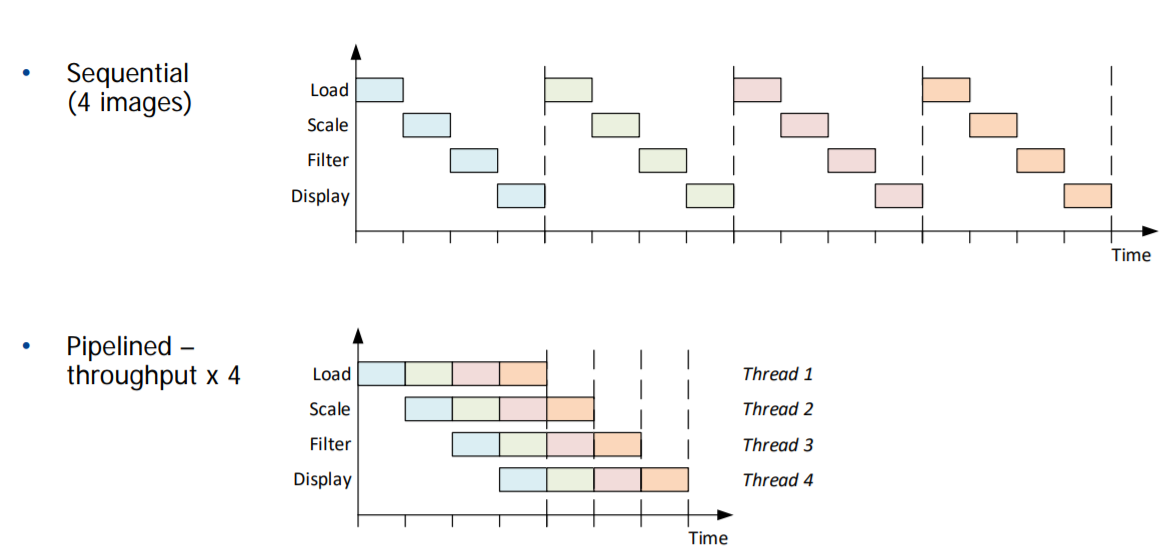
\includegraphics[width = \textwidth]{pipelining.PNG}
\end{figure}
\end{document}
